\section{Neutron Veto Efficiency}
\label{sec:od_analysis_veto_efficiency}
\par
With a measurement of the background rate, the focus now shifts towards determining the veto time window and veto energy threshold that is needed to meet the requirements set out in \autoref{tab:veto_requirements}.
The structure of this section is analogous to \autoref{sec:od_simulation_efficiency}, where an AmLi calibration source is used to determine the veto efficiency.
Given the high rate of ${}^{14}$C seen in the previous section, a veto energy threshold was set to 200 keV.

\subsection{AmLi Veto Efficiency}
\par
For determining the neutron tagging efficiency of the OD, AmLi calibration sources were used.
Three AmLi sources were used simultaneously to improve the neutron flux, each of which were lowered into a separate calibration source tube (CSD).
The activity and locations of each source are summarised in \autoref{tab:amli_source_activities}.

\begin{table}[]
    \centering
    \begin{tabular}{c|c|c}
        CSD & AmLi Source No. & Activity (n/s) \\ \hline
        1   & Source-2        & 13.8$\pm$1.1           \\
        2   & Source-1        & 9.3$\pm$0.7            \\ 
        3   & Source-3        & 11.9$\pm$0.9                
    \end{tabular}
    \caption{AmLi source activities in each calibration source deployment tube (CSD).
             The activity of the sources is from \cite{LZ_TechnicalDesignReview_ref}.}
    \label{tab:amli_source_activities}
\end{table}

\par
Data was taken for a number of hours, with the goal of having a minimum of 1000 nuclear recoil events in the TPC from neutrons.
Three separate sets of data were taken at varying heights in the CSD tubes: 0 mm, 700 mm, and 1400 mm.
These are the same as were presented in \autoref{sec:od_simulation_efficiency}.
During data taking, the S2 Trigger (described in \autoref{sec:lz_detector}) was used, requiring that a large S2 pulse is seen in the TPC.

\par
On the recorded events, a number of analysis cuts were applied to select TPC events of interest.
In addition to the core cuts: single scatters (\textbf{SS}), region of interest (\textbf{ROI}) but adapted slightly to isolate nuclear recoils (\textbf{NR}) and a fiducial cut (\textbf{FID}), two other cuts were applied.
These were based on the S1 pulse (\textbf{S1Cuts}) and the S2 pulse (\textbf{S2Cuts}).
These cuts are a subset of the cuts developed for the SR1 WIMP search \cite{lz_ws_sr1_ref} and are defined as follows:
\begin{itemize}
    \item \textbf{SS}: Single Scatter cut as determined by an interaction finder algorithm. This was tuned on the dataset used here. In an event window, a single scatter is defined if there are only two significant pulses (an S1 and an S2) in the event window. Other pulses can exist, but they must be sufficiently small in size and multiplicity to not be classified as either an S1 or S2.
    \item \textbf{S1Cuts}: This cut ensures that the S1 pulse is not caused by a background process. An example of this is the removal of S1 pulses, where the contribution is primarily from a single PMT, indicating that it is actually an accidental event. S1 pulses which did not have a 3-fold coincidence are also removed.
    \item \textbf{S2Cuts}: This selection is designed to remove events which originate in or near the GXe. If the scatter occurs very close to the GXe then the time separation between the S1 and S2 is sufficiently low that the pulse-finding algorithm cannot separate them. Similarly, GXe scatters would have merged S1 and S2s. Events with a poor position reconstruction (which uses the S2 hit pattern) are also removed this way so as not to influence the \textbf{FID} selection. In combination with the \textbf{S1Cuts}, nonphysical events are removed by the time difference between the pulses.
    \item \textbf{FID}: The inner volume of the TPC is defined in terms of \{$r,z$\}. $r$ is set to a distance [4.0 5.2]~cm from the TPC wall depending on $z$. $z$ was defined by electron drift time of [86, 936.5]~$\mu$s.
    \item \textbf{ROI}: This cut selects scatters with recoil energies akin to a WIMP-nucleon scatter. Only events with an S1$_c$ between [3, 80] are selected and S2 $>$ 600. The latter is to ensure that at least 5 electrons are extracted.
    \item \textbf{NR}: Only events which fall within the 10-90\% quantile band of the nuclear recoil expectation are selected. The NR band used is from DD neutron calibrations described in the \autoref{chap:analysis_eft_work}.
\end{itemize}
These definitions differ from those in \autoref{sec:od_simulation_efficiency} as they are applied to data here rather than simulations.
A summary of the number of events available for this analysis is presented in \autoref{tab:amli_calibration_summary}, and the resulting TPC events are shown in \autoref{fig:amli_tpc_events}.
All OD pulses passing the noise cut and the TPC cuts are shown in \autoref{fig:amli_od_pulsearea_events}.
The peak at $\backsim$400 phd is from n-H captures, which result in the remission of 2.2~MeV $\gamma$s.

\begin{table}[]
    \centering
    \begin{tabular}{c|c|c|c}
        \multirow{2}{*}{z position (mm)} & \multirow{2}{*}{Run IDs}  & \multicolumn2{c}{Number of events}  \\ 
                                         &                           & Acquired    & After all cuts     \\ \hline
        0                                & 8350-8369                 & 5,504,700  & 2252               \\
        700                              & 8304-8317                 & 3,688,200  & 1464               \\ 
        1400                             & 8319-8348                 & 7,041,500  & 3293                
    \end{tabular}
    \caption{Number of events available for analysis from each CDS position.}
    \label{tab:amli_calibration_summary}
\end{table}

\begin{figure}[]%
\centering
\begin{tikzpicture}
\centering
    \begin{axis}[
            ylabel=log$_{10}$(S2$_c$) (phd),
            xlabel=S1$_c$ (phd),
            width=15cm,
            height=8cm,
            xmin=0, xmax=150,
            ymin=2.75, ymax=4.5,
            %ymin=45, ymax=100,
            %minor y tick num=1,
            ]
        \addplot[blue, ]
            table [x=s1c, y=mean]
            {Data/tpc/sr1_er_band.dat};     
        \addplot[blue, dashed]
            table [x=s1c, y=nsig1]
            {Data/tpc/sr1_er_band.dat};     
        \addplot[blue, dashed]
            table [x=s1c, y=psig1]
            {Data/tpc/sr1_er_band.dat};     

        \addplot[red, ]
            table [x=s1c, y=mean]
            {Data/tpc/sr1_nr_band.dat};     
        \addplot[red, dashed]
            table [x=s1c, y=nsig1]
            {Data/tpc/sr1_nr_band.dat};     
        \addplot[red, dashed]
            table [x=s1c, y=psig1]
            {Data/tpc/sr1_nr_band.dat};     
            
        \addplot[black, only marks, mark size=0.25pt]
            table []
            {Data/Neutron_Efficiency/AmLi_Commissioning/amli_s1logs2.dat};
            
    \end{axis}
            
\end{tikzpicture}
    \caption{TPC events which passed all vetoes to attain a high purification of neutron recoils.
             The data points are shown in black, which are from all three AmLi calibration positions.
             The blue and red lines are the electron recoil and nuclear recoil bands respectively. The solid lines are the means whilst the dashed are the 10\% and 90\% quantiles determined from electronic and nuclear recoil calibrations.}
    \label{fig:amli_tpc_events}
\end{figure}
\begin{figure}[]%
\centering
\begin{tikzpicture}
\centering
    \begin{axis}[
            ylabel=Count,
            xlabel=Pulse Area (phd),
            width=15cm,
            height=8cm,
            xmin=0, xmax=2000,
            ymin=0,
            ]
            
        \addplot[black, const plot]
            table[x=bin,y=weight]
            {Data/Neutron_Efficiency/AmLi_Commissioning/amli_od_pulses.dat};

    \end{axis}
            
\end{tikzpicture}
    \caption{Pulse area of all OD pulses associated with single scatter TPC events from AmLi calibration data.}
    \label{fig:amli_od_pulsearea_events}
\end{figure}

\par
In a similar fashion to the previous chapter, the efficiency for vetoing a neutron is defined as:
\begin{equation}
    \epsilon = 1 - \frac{\text{events passing}(\mathbf{SS, S1Cuts, S2Cuts, ROI, NR, FID, Veto})}{\text{events passing}(\mathbf{SS, S1Cuts, S2Cuts, ROI, NR, FID})}
    \label{eq:data_neutron_efficiency}
\end{equation}
The efficiency vs the veto time window is shown in \autoref{fig:commissioning_amli_efficiency_with_bg_rate} for a 200~keV energy threshold.
Overlaid in black is the rate of backgrounds above 200~keV in the OD.
The red dashed line indicates when a 5\% false veto rate is reached, which can be considered the same as the impact on WIMP search live-time.
The point where these two lines cross is the value of the veto window when 5\% of live-time will be vetoed.
For a 200~keV threshold, this is just above 1200~$\mu$s.
With this veto time window, the average neutron tagging efficiency is 84.6$\pm$1.2\%.
This was the OD veto cut used for SR1: 200~keV energy threshold and a 1200~$\mu$s time window.

%In order to maximise the veto efficiency, 1200 $\mu$s was selected as the time window for SR1.
%Complimentary, to the efficiency vs time, \autoref{fig:commissioning_amli_efficiency_per_phd} shows the efficiency vs threshold.

%\begin{figure}[!htbp]%
\centering
\begin{tikzpicture}
\centering
    \begin{axis}[
            ylabel=Efficiency (\%),
            xlabel=Photons Detected (phd),
            width=15cm,
            height=8cm,
            grid=major,
            xmin=0, xmax=100,
            %ymin=45, ymax=100,
            %minor y tick num=1,
            ]
        \addplot[red,
                 error bars/.cd, error bar style={color=red},
                 y dir=both, y explicit, 
                 x dir=both, x explicit,
                 ]
            table [x=bin,y=value, y error minus index=4, y error plus index=5, x error minus index=2, x error plus index=3,]
            {Data/Neutron_Efficiency/AmLi_Commissioning/pos_0_efficiency_per_phd.dat};    
        \addplot[green, 
                 error bars/.cd, error bar style={color=green},
                 y dir=both, y explicit, 
                 x dir=both, x explicit,
                 ]
            table [x=bin,y=value, y error minus index=4, y error plus index=5, x error minus index=2, x error plus index=3,]
            {Data/Neutron_Efficiency/AmLi_Commissioning/pos_700_efficiency_per_phd.dat};             
        \addplot[blue,
                 error bars/.cd, error bar style={color=blue},
                 y dir=both, y explicit, 
                 x dir=both, x explicit,
                 ]
            table [x=bin,y=value, y error minus index=4, y error plus index=5, x error minus index=2, x error plus index=3,]
            {Data/Neutron_Efficiency/AmLi_Commissioning/pos_1400_efficiency_per_phd.dat};    
        \legend{0mm,700mm,1400mm}  
            
    \end{axis}
            
\end{tikzpicture}
    \caption{Efficiency as a function of pulse area}
    \label{fig:commissioning_amli_efficiency_per_phd}
\end{figure}

\begin{figure}[]%
\centering
\begin{tikzpicture}
\centering
    \begin{axis}[
            ylabel=Efficiency (\%),
            xlabel=Time ($\mu$s),
            width=14cm,
            height=8cm,
            grid=major,
            axis y line*=left,
            xmin=0, xmax=1500,
            ymin=45, ymax=100,
            minor y tick num=1,
            legend style = { column sep = 10pt, legend columns = -1,},
            legend pos=north west,
            ]
        \addplot+[red, mark=none, forget plot]
                  table [x=bin,y=value]
                  {Data/Neutron_Efficiency/AmLi_Commissioning/pos_0_od_200kev_efficiency.dat};   
        \addplot[red, only marks, mark size=1.0pt,
                 error bar legend,
                 error bars/.cd, error bar style={color=black},
                 y dir=both, y explicit, 
                 x dir=both, x explicit,
                 ]
            table [x=bin,y=value, y error minus index=4, y error plus index=5, x error minus index=2, x error plus index=3,]
            {Data/Neutron_Efficiency/AmLi_Commissioning/pos_0_od_200kev_efficiency.dat};    
            
        \addplot+[green, mark=none, forget plot]
          table [x=bin,y=value]
          {Data/Neutron_Efficiency/AmLi_Commissioning/pos_700_od_200kev_efficiency.dat};      
        \addplot[green, 
                 only marks, mark size=1.0pt,
                 error bar legend,
                 error bars/.cd, error bar style={color=black},
                 y dir=both, y explicit, 
                 x dir=both, x explicit,
                 ]
            table [x=bin,y=value, y error minus index=4, y error plus index=5, x error minus index=2, x error plus index=3,]
            {Data/Neutron_Efficiency/AmLi_Commissioning/pos_700_od_200kev_efficiency.dat};       
            
        \addplot+[blue, mark=none, forget plot]
          table [x=bin,y=value]
          {Data/Neutron_Efficiency/AmLi_Commissioning/pos_1400_od_200kev_efficiency.dat};         
        \addplot[blue, 
                 only marks, mark size=1.0pt,
                 error bar legend,
                 error bars/.cd, error bar style={color=black},
                 y dir=both, y explicit, 
                 x dir=both, x explicit,
                 ]
            table [x=bin,y=value, y error minus index=4, y error plus index=5, x error minus index=2, x error plus index=3,]
            {Data/Neutron_Efficiency/AmLi_Commissioning/pos_1400_od_200kev_efficiency.dat};    
        \legend{0mm,700mm,1400mm}  
            
    \end{axis}
    \begin{axis}[
            ylabel=False Veto (\%),
            yticklabel pos=right,
            axis y line*=right,
            axis x line=none,
            width=14cm,
            height=8cm,
            %grid=major,
            xmin=0, xmax=1500,
            ymin=0, ymax=50,
            minor y tick num=9,]
        \addplot[domain=0:1500,
            samples=3,
            ]
            {x * 42.5 * 100 / 1000000};
        \iffalse
        \addplot[domain=0:1500,
            samples=3,
            ]
            {x * 95.8 * 100 / 1000000};        
        \addplot[domain=0:1500,
            samples=3,
            ]
            {x * 276.8 * 100 / 1000000};  
        \fi
         \addplot[dashed, mark=none, red] coordinates {(0,5) (1500,5)};
         
        % \node[rotate=24] at (axis cs: 1000,26) {276.8Hz};
        % \node[rotate=11] at (axis cs: 1400,15.5) {95.8Hz};
         \node[rotate=5] at (axis cs: 1400,8) {42.5Hz};
    \end{axis}
            
\end{tikzpicture}
    \caption{Neutron tagging efficiency from AmLi at each height for the 200~keV phe threshold.
    The horizontal dashed line is the 5\% impact on live-time requirement.
    The black line is the 200~keV background rate in the OD.}
    \label{fig:commissioning_amli_efficiency_with_bg_rate}
\end{figure}

\par
In \autoref{fig:sr1_vetoed_events}, the effect of the OD veto is illustrated on the SR1 WIMP search data in an extended \textbf{ROI}.
Points marked in black are events which passed all other analysis cuts and were not vetoed by the OD.
Points marked in green are events which passed all other analysis cuts but were vetoed by the OD.
Overlaid are the ER and NR bands.
None of the events vetoed by the OD are near the NR band.
This indicates that all events which were vetoed are not neutrons but rather backgrounds in the OD.
Several events which weren't vetoed by the OD are in the NR band.
This will become clear in the following chapter.
These events are not neutrons but are consistent with ER leakage into the NR band.
The lack of seeing any neutrons in this dataset is consistent with the low neutron rate from ($\alpha$,$n$) and spontaneous fission from the detector materials \cite{LZ_TechnicalDesignReview_ref}.

\begin{figure}[]%
\centering
\begin{tikzpicture}
\centering
    \begin{axis}[
            ylabel=Log10(S2) (phd),
            xlabel=S1 (phd),
            width=15cm,
            height=8cm,
            xmin=0, xmax=600,
            ymin=3, ymax=5,
            %ymin=45, ymax=100,
            %minor y tick num=1,
            ]
            
        \addplot[black, only marks, mark=+]
            table []
            {Data/Neutron_Efficiency/AmLi_Commissioning/s1s2_passed_od_veto_in_fid.dat};    
        \addplot[green, only marks, mark=o]
            table []
            {Data/Neutron_Efficiency/AmLi_Commissioning/s1s2_failed_od_veto_in_fid.dat};
        
        \addplot[blue, ]
            table [x=s1c, y=mean]
            {Data/tpc/sr1_er_band.dat};     
        \addplot[blue, dashed]
            table [x=s1c, y=nsig1]
            {Data/tpc/sr1_er_band.dat};     
        \addplot[blue, dashed]
            table [x=s1c, y=psig1]
            {Data/tpc/sr1_er_band.dat};     

        \addplot[red, ]
            table [x=s1c, y=mean]
            {Data/tpc/sr1_nr_band.dat};     
        \addplot[red, dashed]
            table [x=s1c, y=nsig1]
            {Data/tpc/sr1_nr_band.dat};     
        \addplot[red, dashed]
            table [x=s1c, y=psig1]
            {Data/tpc/sr1_nr_band.dat};     
            
    \end{axis}
            
\end{tikzpicture}
    \caption{TPC events vetoed by the OD. In Red are events which passed all cuts including the OD veto. In Blue are events which passed all cuts except the OD veto.}
    \label{fig:sr1_vetoed_events}
\end{figure}

\par
Turning back to the veto efficiency, it is lower than the 95\% requirement, at 84.6\%.
As such requirement R-160001 is not satisfied.
However, in SR1, the impact on live-time in the \textbf{ROI} was 4.99\%, and so requirement R-160005 is met.
It may, in future, be possible to reduce the impact on live-time by un-vetoing OD events if it is possible to determine the cause of light.
The most obvious starting point for this is to find back-to-back $\alpha$-decays, such as was done in the previous section.

\par
Looking at the shape of the efficiency curve in \autoref{fig:commissioning_amli_efficiency_with_bg_rate}, and compared to the simulation result (\autoref{fig:simulated_amli_full_propagation_efficiency} in the previous chapter), the measured efficiency is lower than was expected.
With a 200~keV threshold and a 1200 $\mu$s window, the simulation result predicts an efficiency of 91.8\%, whilst in data the measured efficiency is 84.6\%.
Additionally, the shape of the curves appear to be slightly different.
This indicates that the neutron propagation is not modelled accurately in the simulation, and prompted the study detailed in the next section.

\subsection{Neutron Propagation}
\par
To study the neutron propagation differences between simulation and data, neutron captures were used.
In order to do this, a high-purity sample of neutrons is needed, and ideally, high statistics.
${}^{252}$Cf calibrations were deemed the most appropriate as the neutron rate is 430 per second. 
It is deployed in the calibration source tube in the same manner as the AmLi source, so neutrons will travel from the OCV towards the OD.
\par
${}^{252}$Cf decays via spontaneous fission, releasing on average 3.7 neutrons each time \cite{californium252_ref}.
During the fission, a number of $\gamma$s with a combined energy of up to 10 MeV are also released.
The vast majority of these $\gamma$s are released within the first 100 ns of the fission event \cite{cf252_fission_ref,californium_spectra_ref}.
Given that the $\gamma$s are released close in time to when the neutrons are released, they can be used to tag the neutron creation time, $t_0$.
The waveforms in each detector from an event during the ${}^{252}$Cf calibration run is shown in \autoref{fig:cf252_event_viewer}.
There is a signal in all three detectors at the same time which is from the $\gamma$s.
The later pulses in the OD are then from neutron capture, two captures in this case.
%\begin{figure}[!htbp]
%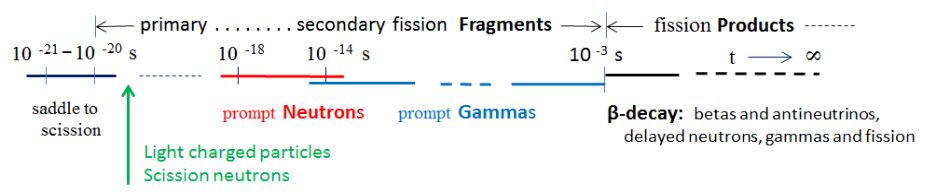
\includegraphics[width=13cm]{Figures/NeutronCaptureTime/fission_fragment_times.png}
%\centering
%\caption{Emission time-frame of fission components. Adapted from \cite{cf252_fission_ref}}
%\label{fig:fission_fragments_time}
%\end{figure}


\begin{figure}[]
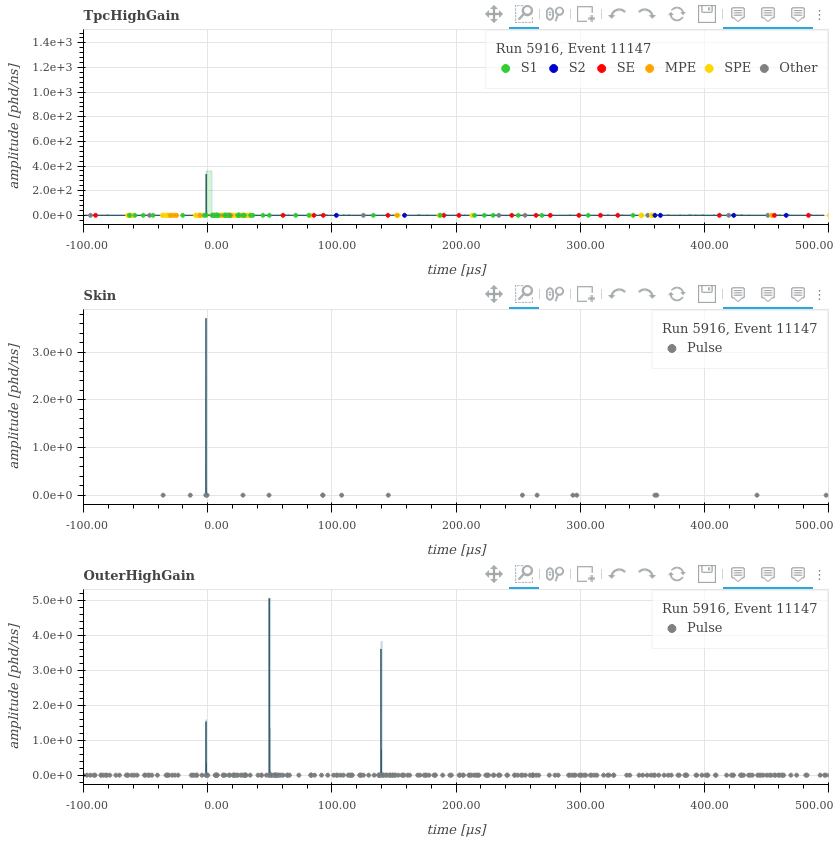
\includegraphics[width=\textwidth]{Figures/NeutronCaptureTime/cf252_eventviewer_5916.png}
\centering
\caption{Example event from ${}^{252}$Cf calibration run showing the $\gamma$s causing coincident pulses in each detector followed by two neutrons being captured in the Outer Detector.}
\label{fig:cf252_event_viewer}
\end{figure}

\par
The ${}^{252}$Cf datasets selected for this study were from runs with a single source in CSD-1 at the 700~mm level.
An event was only considered if a triple coincidence was observed, defined as both the Skin and TPC detectors seeing light within [-200, 200]~ns of a pulse seen in the OD.
The largest triple coincidence pulse in an event was taken to be $t_0$.
Given that a neutron capture on gadolinium will release $\gamma$s with a combined energy of 8 MeV, there is a probability of some of these pulses being from a neutron capture.
However, it is unlikely that this will result in a triple coincidence due to the starting location of the post-capture $\gamma$s.
To avoid backgrounds contributing, an energy threshold in the OD of 250~keV was used.
The spectra of OD pulses which make up the $t_0$ event are shown in \autoref{fig:cf252_pulse_selection}.
The OD pulses both before and after $t_0$ are also shown.
%The shapes are quite different between each selection.
The peak around 450~phd in the before and after $t_0$ distributions are the 2.2~MeV $\gamma$ from n-H captures, and it is missing from the $t_0$ distribution as these are multiple $\gamma$ events.
%The number of events after $t_0$ is consistent with neutrons being captured some time after the fission $\gamma$s are emitted.
Some of the pulses after $t_0$ are background events.
To remove these, only the largest pulse in an event was used for the capture time.
This distribution is shown in \autoref{fig:cf252_gd152_captures}.
Finally, only pulses above 600 phd were considered.
This ensures that captures in other H-rich media were not included (such as in the acrylic tanks and foam) to ensure a high purity of n-Gd captures.
The final set of pulses after $t_0$ are neutrons which capture on gadolinium and so in the GdLS.

\begin{figure}[]%
\centering
\begin{tikzpicture}
\centering
    \begin{axis}[
            ylabel=Count,
            xlabel=Pulse Area (phd),
            width=15cm,
            height=8cm,
            grid=major,
            xmin=0, xmax=2500,
            ymode=log,
            %ymin=45, ymax=100,
            %minor y tick num=1,
            ]
        \addplot[red, only marks, mark size=1.0,
                 error bar legend,
                 error bars/.cd, error bar style={color=black},
                 y dir=both, y explicit, 
                 x dir=both, x explicit,
                 ]
            table [x=pulsearea,y=weight, x error=xerror, y error=yerror]
            {Data/cf252/cf252_od_pulses_before400ns.dat};    
        \addplot[green, only marks, mark size=1.0,
                 error bar legend,
                 error bars/.cd, error bar style={color=black},
                 y dir=both, y explicit, 
                 x dir=both, x explicit,
                 ]
            table [x=pulsearea,y=weight, x error=xerror, y error=yerror]
            {Data/cf252/cf252_od_pulses_within400ns.dat};           
        \addplot[blue, only marks, mark size=1.0,
                 error bar legend,
                 error bars/.cd, error bar style={color=black},
                 y dir=both, y explicit, 
                 x dir=both, x explicit,
                 ]
            table [x=pulsearea,y=weight, x error=xerror, y error=yerror]
            {Data/cf252/cf252_od_pulses_after400ns.dat};
        \legend{Before 400ns,Within 400ns,After 400ns}  
            
    \end{axis}
            
\end{tikzpicture}
    \caption{Pulse Distribution depending upon when the tagging pulse was.}
    \label{fig:cf252_pulse_selection}
\end{figure}

\begin{figure}[!htbp]%
\centering
\begin{tikzpicture}
\centering
    \begin{axis}[
            ylabel=Count,
            xlabel=Photons Detected (phd),
            width=15cm,
            height=8cm,
            grid=major,
            xmin=0, xmax=2500,
            %ymin=45, ymax=100,
            %minor y tick num=1,
            ]
        \addplot[black, only marks, mark size=1.0,
                 error bars/.cd, error bar style={color=black},
                 y dir=both, y explicit, 
                 x dir=both, x explicit,
                 ]
            table [x=pulsearea,y=weight, x error=xerror, y error=yerror]
            {Data/cf252/cf252_od_largest_after400ns.dat}; 
            
    \end{axis}
            
\end{tikzpicture}
    \caption{Largest OD pulse in an event window 400ns after the first coincidence pulse.}
    \label{fig:cf252_gd152_captures}
\end{figure}

\par
The time difference between the capture pulse and $t_0$ is shown in \autoref{fig:cf252_gd_capture_time}.
A fit (following \autoref{eq:neutron_capture_time}) was performed and found that two exponentials were best, with $\tau_0 = 31.39 \pm 0.4\mu$s and $\tau_1 = 124.5 \pm 1.7\mu$s, with a $\chi^2$/ndof$=0.821$.
Included as well is the result of simulated ${}^{252}$Cf fission neutrons from the same starting position.
$\tau_0$ is in good agreement with the simulations, indicating that once the neutrons reach the GdLS they are captured quite fast.
However, neutrons are clearly being held up in other regions of the detector, somewhere between the calibration tube and the GdLS that isn't simulated.
The simplest explanation is that water has gotten in between the OCV and acrylic tanks.
The foam installed between the OCV and the OD acrylic tanks (documented in \autoref{sec:od_construction_sec}) was installed to displace water, but it is possible that the foam has saturated with water.

\begin{figure}[]%
\centering
\begin{tikzpicture}
\centering
    \begin{axis}[
            ylabel=Count,
            xlabel=Capture Time ($\mu$s),
            width=15cm,
            height=8cm,
            grid=major,
            ymode=log,
            xmin=-10,xmax=1000,
            ymin=1,
            %minor y tick num=1,
            ]
        \addplot[black, only marks, mark size=0.5,
                 error bars/.cd, error bar style={color=black},
                 y dir=both, y explicit, 
                 x dir=both, x explicit,
                 ]
            table [x=time,y=weight, x error=xerror, y error=yerror]
            {Data/cf252/cf252_gd_capture_time.dat}; 
            
        \addplot[red,
                 domain=15:1500,
                 ]
            {2305 * exp(-x/30.5) + 342 * exp(-x/125.2) + 0.9663}; 
            
        \addplot[blue,
                 domain=15:1500,
                 ]
            {2294 * exp(-x/31.2) + 235 * exp(-x/70.1) + 11.94 * exp(-x/176.4)}; 
            
    \end{axis}
            
\end{tikzpicture}
    \caption{Pulse Distribution depending upon when the tagging pulse was.
             In red is the best fit from 2 exponential decays.
             In blue is the expected neutron capture time.}
    \label{fig:cf252_gd_capture_time}
\end{figure}

\par
Water ingress into foam has been well studied  with the industrial measures of water absorption defined as via diffusion and submersion \cite{foam_with_water_ref}.
The effectiveness of any foam type to keep water out is based on a number of factors, including density and, most importantly, if the structure is closed or open\footnote{in terms of the cells which make up the foam structure. Open-cell foams are softer and more flexible as each cell is open to the atmosphere. Closed cell foams are firmer, with the majority of cells being closed to the atmosphere.} \cite{mechanical_properties_of_foam_ref}.
An example of water ingress is shown in \autoref{fig:foam_mri_water_ingress}.


\begin{figure}[]
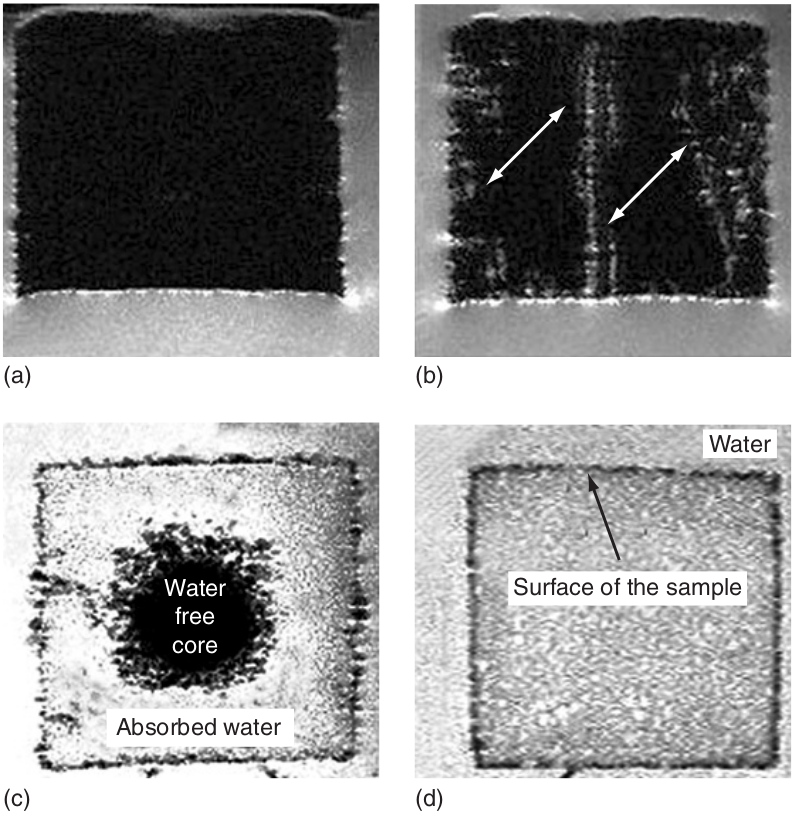
\includegraphics[width=0.5\textwidth]{Figures/NeutronCaptureTime/foam_water_absorption.png}
\centering
\caption{Magnetic resonance images of 30 mm cube samples of polyurethane foam for two types of different foam of the same density, 0.3 g m${}^{-3}$: a closed cell foam (top) and an open cell foam (bottom).
(a) closed cell foam after 8 hours. (b) closed cell foam after 63 hours.
(c) open cell foam after 8 hours. (d) open cell foam after 72 hours.
Images from \cite{foam_mri_data_ref}.
}
\label{fig:foam_mri_water_ingress}
\end{figure}


\par
The foam installed around the OCV (green Styrodur foam mentioned in \autoref{sec:od_construction_sec}) is a closed cell foam expanded using CO$_2$, foam 3000 CS in \cite{styrodur_water_ingress_ref}.
As such, the foam is expected to experience a 0.7\% volume ingress of water due to long-term submersion and 5\% volume ingress of water from diffusion.
Long-term refers to a 28-day test as is the industry standard\footnote{see BS EN ISO 16535 (previously BS EN 12087) and BS EN ISO 16536 (previously BS EN 12088)}.
These values do not necessarily map onto how the foam was used in the OD, particularly given that water pressure is not considered in the industry tests and the submersion duration is significantly less than the LZ foam has already been exposed to.
The other two foams, HandiFoam\textsuperscript{\textregistered} and white polyethylene foam, are also closed-cell and have slightly different water ingress results \cite{handifoam_water_ingress_ref, white_foam_ref}. 
\par
In order to probe this hypothesis, a test was conducted to observe what happens to this foam (and the water) during submersion.
An example of each piece of foam used was placed in de-ionised water with nitrogen bubbling through it. 
The water resistivity was measured every few hours to monitor the water purity.
The result over the first week of running is shown in \autoref{fig:od_foam_degredation}.
What is observed during this period is the water becoming contaminated with ions from the foam from outgassing, causing the resistivity to increase.
This can then be replaced by water.
Over a longer period of study, it will be possible to measure the water saturation by weight.
Ideally, a test will be conducted using foam pieces shaped to the same dimensions as those used in the installation, as the rate at which water ingress occurs will depend upon the surface area.
\par
In relation to LZ, this has two consequences.
Firstly these ions can circulate throughout the OD water and contribute to the low energy background rate in the OD.
Secondly, this will reduce the number of neutrons which reach the GdLS and increase the time it takes for a neutron to be captured.
In \autoref{fig:data_vs_sim_gd_capture_time} are the simulated neutron capture time in GdLS assuming the extreme case of all of the foam around the OCV being directly replaced with water, and the more realistic scenario of the foam being filled with 5\% (by volume) with water.
The 5\% saturation case provides a better match to the observed capture time.

\par
The 5\% saturation case provides a better fit up to a capture time of 300~$\mu$s, but above this does not describe the data well.
It is possible that other isotopes are playing an important role in the neutron thermalisation.
Both Oxygen and Carbon are around the GdLS, in both the foam and acrylic.
Although both of these have a much lower neutron cross-section, it is possible contributing to the extended neutron capture times.
Further studies are needed to determine what other differences there may be between the simulated neutron propagation and what is observed, but water ingress appears to be the dominant factor.
A future search should focus on the ratio of n-H captures to n-Gd captures, as this will allow for the water ingress theory to be tested.

\begin{figure}[]%
\centering
\begin{tikzpicture}
\centering
    \begin{axis}[
            xlabel=Time (hours),
            ylabel=Resistivity (mS/cm),
            width=15cm,
            height=8cm,
            grid=major,
            xmin=-1, xmax=250,
            legend style={at={(0.95,0.5)},anchor=east},
            %ymin=45, ymax=100,
            %minor y tick num=1,
            ]
        \addplot[green, only marks,
                 error bars/.cd, error bar style={color=black},
                 y dir=both, y explicit, 
                 ]
            table [x=time,y=di,y error=error]
            {Data/cf252/foam_in_di_water.dat}; 
        \addplot[blue, only marks,
                 error bars/.cd, error bar style={color=black},
                 y dir=both, y explicit, 
                 ]
            table [x=time,y=foam,y error=error]
            {Data/cf252/foam_in_di_water.dat}; 
        \addplot[red, dashed,
                 domain=-10:750,
                 samples=3]
                {1};
            
        \legend{Control, Foam,};
    \end{axis}
            
\end{tikzpicture}
    \caption{Measure of water purity from foam used in the OCV.
             Both the Control (just water) and the Foam (water with foam pieces) were under $N_2$ purge for the duration of the data taking.
             The dashed red line indicated the Type 2 DI water limit.}
    \label{fig:od_foam_degredation}
\end{figure}

\begin{figure}[]%
\centering
\begin{tikzpicture}
\centering
    \begin{axis}[
            ylabel=Count (Arb.),
            xlabel=Capture Time ($\mu$s),
            width=15cm,
            height=8cm,
            grid=major,
            ymode=log,
            xmin=-10,xmax=800,
            ymin=1e-3, ymax=5,
            %minor y tick num=1,
            ]
        \addplot[black, only marks, mark size=0.5,
                 error bars/.cd, error bar style={color=black},
                 y dir=both, y explicit, 
                 ]
            table [x=time,y=weight, y error=yerror]
            {Data/cf252/cf252_gd_capture_time_normed.dat}; 
            
        \addplot[red, const plot]
            table [x=time,y=weight]
            {Data/cf252/amli_0mm_default.dat}; 
            
        \addplot[green, const plot]
            table [x=time,y=weight]
            {Data/cf252/amli_0mm_water_saturated.dat}; 

        \addplot[blue, const plot]
            table [x=time,y=weight]
            {Data/cf252/amli_0mm_water.dat}; 
            
    \end{axis}
            
\end{tikzpicture}
    \caption{Neutron capture time on Gadolinium in the OD. The observed capture time from ${}^{252}$Cf is shown in black. In red is the expected capture time from simulation. In green is the capture time if the foam has been saturated with water up to 5\% of its volume. In blue is the capture time if all foam around the OCV has been replaced with water. Each distribution has been normalised the maximum value.}
    \label{fig:data_vs_sim_gd_capture_time}
\end{figure}